\documentclass[12pt,a4paper]{article}
\usepackage[utf8]{inputenc}
\usepackage[brazilian]{babel}
\usepackage[skip=1.2\baselineskip]{parskip}
\usepackage{amsmath}
\usepackage{amsfonts}
\usepackage{amssymb}
\usepackage{bm}
\usepackage{geometry}
\usepackage{graphicx}
\usepackage{makecell}
\usepackage{tcolorbox}
\usepackage{tikz}
\usepackage{setspace}
\usepackage{tabularx}
\usepackage{hyperref}
\usepackage[all]{nowidow}

\setstretch{1.2} 
\tcbuselibrary{breakable, skins}

\geometry{top=2cm, bottom=2cm, left=2.5cm, right=2.5cm}

\hypersetup{
	colorlinks=true,
	linkcolor=blue,
	filecolor=magenta,      
	urlcolor=blue,
	pdftitle={Critérios de Divisibilidade},
}

\newtcolorbox{meudestaque}[1][]{
	colback=gray!10, 
	colframe=black, 
	arc=0mm,        
	sharp corners,
	boxrule=0.5pt,
	#1
}

% Caixa de destaque padronizada
\newtcolorbox{meudestaque2}[1][]{
	enhanced,
	breakable,
	colback=white,
	colframe=black,
	opacityframe=1,         % Garante que a borda seja 100% opaca
	arc=0mm,
	sharp corners,
	boxrule=0.5pt,
	% Reforço das linhas de quebra com espessura e cor explícitas
	toprule at break=0.5pt,
	bottomrule at break=0.5pt,
	colframe=black,         % Reitera a cor para evitar tons acinzentados
	#1
}

\begin{document}
	
	% --- CABEÇALHO ---
	\begin{tcolorbox}[
	enhanced, 
	colback=white, 
	colframe=black, 
	boxrule=2pt,
	left=0pt, 
	right=0pt,
	top=5pt,
	bottom=5pt
	]
	\noindent
		\begin{minipage}[c]{0.25\textwidth}
			\centering
			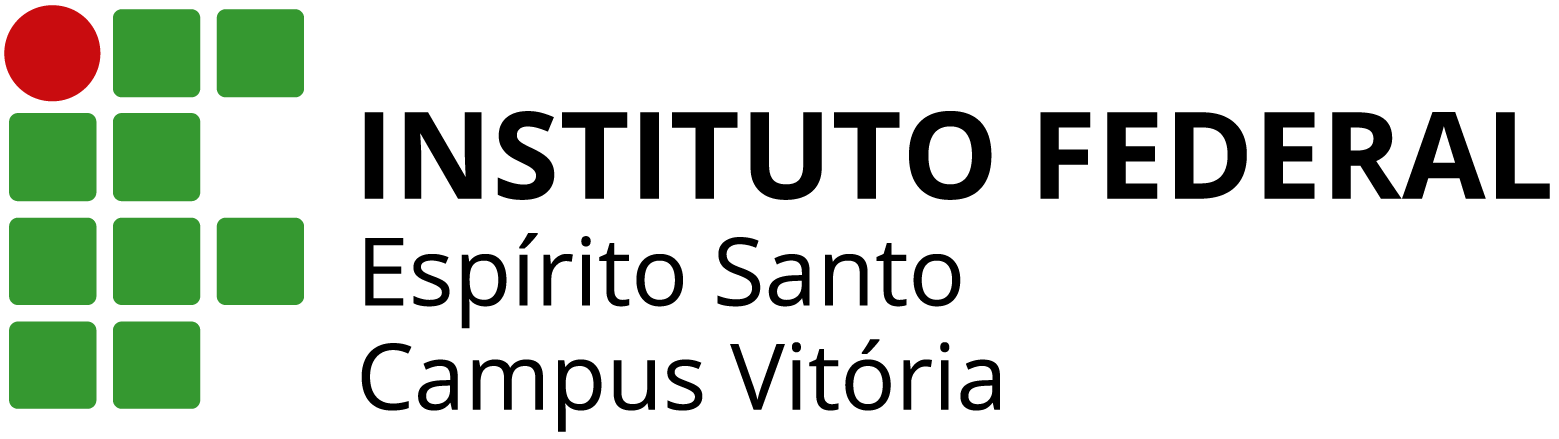
\includegraphics[width=4.5cm]{ifes.png} 
		\end{minipage}
		\begin{minipage}[c]{0.70\textwidth}
			\centering
			\textbf{Investigando Critérios de Divisibilidade}\\
			\textbf{Licenciatura em Matemática}\\
			Professor: \textbf{Alex Jordane}
		\end{minipage}
	\end{tcolorbox}
	
	\vspace{\fill}
	
		A divisibilidade é uma ideia que pode nos ajudar a compreendermos a estrutura dos números naturais. Vamos tratar de algumas ideias que envolvem procedimentos que nos permitem verificar se um número $N$ é divisível por outros números. Vamos focar nos números primos e em alguns outros naturais produtos de dois primos.
		
		Vamos organizar os procedimentos de verificação em três grupos: (\ref{sec:posicao}) procedimentos pela posição; (\ref{sec:soma}) procedimentos pela soma de algarismos; e (\ref{sec:decomp}). procedimentos por decomposição de números. Em alguns momentos poderemos combinar mais de um desses procedimentos.
		
		Como estaremos tratando de procedimentos, iremos dar uma atenção aos processos matemáticos que justificam os procedimentos. Reforçamos assim que, \textbf{mais do que ``decorar'' os procedimentos, é importante compreeder os processos matemáticos envolvidos}.
		
		Bons estudos!
		
		\vspace{\fill}
		
		\footnotesize
		\texttt{Esta é uma segunda versão do material, editada em 17/08/2026.}\\
		\texttt{Este material foi elaborado em colaboração com a inteligência artificial Gemini, versão 3.1 Pro.} \\		
		\texttt{O compartilhamento e a reprodução deste material são permitidos, desde que a fonte e a autoria sejam citadas.}  \\		
		\texttt{Esta obra está licenciada com uma Licença Atribuição-NãoComercial-SemDerivações 4.0 Brasil.}
		\begin{center}
			
\includegraphics[width=4cm]{CC.png}
		\end{center}
		
		\newpage
		
		\section*{Notações de Números Inteiros}
		
		Antes de iniciarmos a discussão sobre os procedimentos, cabe uma explicação sobre as notações de um número inteiro usadas neste material. Vamos sempre chamar o número que queremos descobrir seus divisores de $N$. Iremos também notar o número $N$ a partir dos algarismos que o compõem.
		
		\subsection*{Primeira notação}
		\label{sub:1notacao}
		Imaginemos então que $N = 1234$. $N$ é formado pelos algarismos 1, 2, 3 e 4, da maior para a menor ordem, ou seja 1 milhar, 2 centenas, 3 dezenas e 4 unidades. 
				
		Nesta primeira forma de denotar o número $N$, vamos nomear o algarismo da maior ordem (no caso milhar, ou quarta ordem) de $a$, o da segunda maior ordem (no caso centenas, ou terceira ordem) de $b$, e assim sucessivamente até o algarismo das unidades (primeira ordem).
		
		De forma geral, podemos escrever que $N = abcd$. Para não confundir com uma multiplicação $a$ por $b$ por $c$ por $d$, sempre que estivermos tratando de multiplicação utilizaremos o operador multiplicativo ($\cdot$).
		
		Voltemos ao nosso número $N = 1234$. Então podemos escrever que
		$$N = 1000 \cdot 1 + 100 \cdot 2 + 10 \cdot 3 + 4$$
		Neste caso teremos $a = 1$, $b = 2$, $c = 3$ e $d = 4$. Generalizando em função de $a$, $b$, $c$ e $d$:		
		\begin{align}
			N &= 1000 \cdot a + 100 \cdot b + 10 \cdot c + d
			\label{eq:not1}
		\end{align}		
		Cabe ressaltar que para um número maior, por exemplo, $N = 46978$, precisaríamos de 5 letras para representar cada um dos 5 algarismo. Logo $N = abcde$, com $a = 4$, $b = 6$, $c = 9$, $d = 7$ e $e = 8$.
		
		\subsection*{Segunda notação}
		
		Nesta segunda forma de denotar o número $N$, vamos destacar o ``ultimo'' algarismo, ou seja o algarismo da menor ordem (unidades), do restante.
		
		De forma geral, podemos escrever que $N = ab$, com $b$ representando o algarismos das unidades e $a$ os demais algarismos. 
		
		Voltemos ao nosso número $N = 1234$. Então podemos escrever que 
		$$N = 10 \cdot 123 + 4$$ 
		Neste caso teremos $a = 123$ e $b = 4$. Generalizando em função de $a$ e $b$:
		\begin{align}
			N &= 10 \cdot a + b
			\label{eq:not2}
		\end{align}		
		Cabe ressaltar que para um número maior, por exemplo, $N = 46978$, só muda o valor de $a$ para representar os 4 algarismos de maior ondem. Logo $N = ab$, com $a = 4697$ e $b = 8$.
		
		\subsection*{Terceira notação}
		
		Nesta terceira forma de denotar o número $N$, vamos destacar os 2 ``últimos'' algarismos, ou seja o algarismo das unidades e das dezenas, do restante.
		
		Como na segunda notação, de forma geral, podemos escrever que $N = ab$, com $b$ representando os algarismos das unidades e dezenas e $a$ os demais algarismos. 
		
		Voltemos ao nosso número $N = 1234$. Então podemos escrever que 		
		$$N = 100 \cdot 12 + 34$$ 		
		Neste caso teremos $a = 12$ e $b = 34$. Generalizando em função de $a$ e $b$:		
		\begin{align}
			N &= 100 \cdot a + b
			\label{eq:not3}
		\end{align}		
		Cabe ressaltar que para um número maior, por exemplo, $N = 46978$, só muda o valor de $a$ para representar os 3 algarismos de maior ondem. Logo $N = ab$, com $a = 469$ e $b = 78$.
		
		\subsection*{Outras notações}
		
		A partir das ideias utilizadas na segunda (\ref{eq:not2}) e na terceira (\ref{eq:not3}) notações podemos criar outras notações destacando $b$ como 3, 4 ou quantos ``últimos'' algarismos quisermos.
		
		\section{Procedimentos pela Posição}
		\label{sec:posicao}
		Os procedimentos pela posição nos permitem identificar a divisibilidade pelos números primos 2 e 5, e por seus produtos. 
		
		\subsection{Divisibilidade por 2 e por 5}
		\label{sub:2_5}
		O procedimentos que tratam da identificação da divisibilidade por 2 e por 5 se focam exclusivamente do algarismo das unidades. Logo usaremos a segunda notação (\ref{eq:not2}): $N = 10 \cdot a + b$ e nos atentaremos a $b$. 
		
		\subsubsection{Divisibilidade por 2}
		Para que um número seja divisível por 2, que é o memo que dizer que o número é par, basta identificarmos o algarismos das unidades $b$. Se $b$ é divisível por 2, ou seja, se $b$ é par, $N$ também será divisível por 2, ou seja, também será um número par.
		
		Apesar se parecer meio óbvio esse procedimento, vamos apresentar, como já tratamos, as justificativas desse procedimento.
		
		\textbf{Jutificativa:}\\
		Consideremos um número $N$ qualquer, sua representação será $N = ab$, de acordo com a notação \ref{eq:not2}.		
		$$N = 10 \cdot a + b$$
				
		Para que $N$ seja divisível por 2, ambas as parcelas ($10 \cdot a$ e $b$) devem ser divisíveis por 2. Mas, como $10 \cdot a$ é divisível por 10 e 10 é divisível por 2, basta que $b$ seja divisível por 2 para que $N$ também seja divisível por 2. Os números menores que 10 (algarismos) divisíveis por 2 são 0, 2, 4, 6 e 8, logo concluímos que
		
		\begin{meudestaque}
			Se $b = 0$, $b = 2$, $b = 4$, $b = 6$ ou $b = 8$, $N$ é divisível por 2.
		\end{meudestaque}
		
		\subsubsection{Divisibilidade por 5}
		
		Como na divisibilidade por 2, para identificar a divisibilidade por 5, basta identificarmos o algarismos das unidades $b$. Se $b$ é divisível por 5, $N$ também será divisível por 5.
		
		Vamos usar a mesma lógica.
		
		\textbf{Jutificativa:}\\
		Vamos usar $N = ab$, de acordo com a notação \ref{eq:not2}.		
		$$N = 10 \cdot a + b$$		
		Para que $N$ seja divisível por 5, ambas as parcelas ($10 \cdot a$ e $b$) devem ser divisíveis por 5. Mas, como $10 \cdot a$ é divisível por 10 e 10 é divisível por 5, basta que $b$ seja divisível por 5 para que $N$ também seja divisível por 5. Os números menores que 10 (algarismos) divisíveis por 5 são 0 e 5, logo concluímos que 
		
		\begin{meudestaque}
			Se $b = 0$ ou $b = 5$, $N$ é divisível por 5.
		\end{meudestaque}
		
		\subsection{Divisibilidade por múltiplos de 2 e de 5}
		\label{sub:m2_5}
		Nesta seção vamos tratar dos números divisíveis por 10 ($2 \cdot 5$), por 4 ($2 \cdot 2$) e ainda vamos dar algumas dicas para os números divisível por potências de 10: 100, 1000, $\cdots$ e por potências de 2: 8, 16, $\cdots$.
		
		\subsubsection{Divisibilidade por 10}
		Para que um número seja divisível por 10, ele precisa ser divisível, simultaneamente por 2 e por 5, visto que $10 = 2 \cdot 5$.
		
		\textbf{Jutificativa:}
		\begin{itemize}
			\item Os números divisíveis por 2 devem ter $b$ pertencendo ao conjunto $A = \{0, 2, 4, 6, 8\}$.
			\item Os números divisíveis por 5 devem ter $b$ pertencendo ao conjunto $B = \{0, 5\}$.
			\item Os números divisíveis por 10 devem ter $b$ pertencendo ao conjunto $C = A \cap B$, ou seja $C = \{0\}$.			
		\end{itemize}
				\begin{meudestaque}
			Se $b = 0$, $N$ é divisível por 10.
		\end{meudestaque}
		
		\newpage
		
		\subsubsection{Divisibilidade por 4}
		Para os números divisíveis por 4 vamos usar a notação \ref{eq:not3} ($b$ é formado pelos algarismos das dezenas e da unidade): $N = 100 \cdot a + b$.
		
		Como nos procedimentos de divisibilidade por 2 e 5, a parcela $100 \cdot a$ é divisível por 4, pois 100 é divisível por 4. Logo:
		
		\begin{meudestaque}
			Se $b$ for divisível por 4, $N$ é divisível por 4.
		\end{meudestaque}
		
		Para saber se $b$ é divisível por 4, basta dividir $b$ por 2, se o resultado também for divisível por 2, $b$ será divisível por 4.
		
		\subsubsection{Divisibilidade por potências de 10}
		
		Não vamos nos alongar aqui, mas para que um número $N$ seja divisível por $10^x$, basta que tenhamos ``$x$'' zeros nos ``últimos'' algarismos. Por exemplo: 10000 é divisível por $10 = 10^1$ (``termina'' com 1 zero), por $100 = 10^2$ (``termina'' com 2 zeros), por $1000 = 10^3$ (``termina'' com 3 zeros) e por $10000 = 10^4$ (``termina'' com 4 zeros)
		
		\subsubsection{Divisibilidade por potências de 2}
		
		Vamos começar pensando em $8 = 2^3$ e vamos usar as ideias da divisibilidade por $4 = 2^2$.
		
		Se para $4 = 2^2$ tomamos a notação \ref{eq:not3} (separando os 2 ``ultimos'' algarismos), para $8 = 2^3$ vamos considerar outra notação: $N = 1000 \cdot a + b$, ou seja, vamos isolar os 3 ``últimos'' algarismos. Como $1000 \cdot a$ é divisível por 8 $\left( \frac{1000}{8} = 125 \right)$, basta que $b$ seja divisível por 8. Podemos fazer o mesmo processo na divisibilidade por 4: divida $b$ por 2, em seguida divida o resultado por 2 e, se o resultado dessa última operação for divisível por 2, $N$ será divisível por 8.
		
		Para as demais potências de 2, do tipo $2^x$, basta tomarmos os ``últimos $x$'' algarismos. Para a divisibilidade por $16 = 2^4$, tome os 4 últimos algarismos e assim por diante.
		
		\section{Procedimento pela Soma de Algarismos}
		\label{sec:soma}
		
		Para que um número seja divisível por 3, ou por 9, basta que a soma de seus algarismos também seja divisível por 3, ou por 9. Se a identificação da divisibilidade por 3, ou por 9, desse resultado for ainda difícil, some novamente seus algarismos e assim até chegar a número fácil de identificar a divisibilidade por 3, ou por 9.
		
		\textbf{Exemplo:} Vamos voltar ao nosso número $N = 1234$, $1+2+3+4 = 10$. Como 10 não é divisível por 3, 1234 não é divisível por 3 (muito menos por 9, visto que para ser divisível por 9, ele precisa, necessariamente, ser divisível por 3).
		
		\newpage
		
		\subsection{Divisibilidade por 3}
		
		\textbf{Justificativa:}\\
		Usaremos a notação \ref{eq:not1}: $N = 1000 \cdot a + 100 \cdot b + 10 \cdot c + d$. 
		
		Podemos escrever essa notação de outra forma:
		\begin{align*}
			N &= 999 \cdot a + a + 99 \cdot b +b + 9 \cdot c + c + d\\
			N &= 999 \cdot a + 99 \cdot b + 9 \cdot c + a + b + c + d\\
			N &= (999 \cdot a + 99 \cdot b + 9 \cdot c) + (a + b + c + d)\\
			N &= 3 \cdot (333 \cdot a + 33 \cdot b + 3 \cdot c) + (a + b + c + d)\\
		\end{align*}
		Assim, podemos concluir que a parcela $3 \cdot (333 \cdot a + 33 \cdot b + 3 \cdot c)$ é divisível por 3.
		
		Logo
		
		\begin{meudestaque}
			Se $a+b+c+d$ for divisível por 3, $N$ é divisível por 3.
		\end{meudestaque}
		
		O mesmo poderemos fazer para números com 5, 6 ou mais algarismos.
		
		\subsection{Divisibilidade por 9}
		
		\textbf{Justificativa:}\\
		Partindo da expressão:
		$$N = (999 \cdot a + 99 \cdot b + 9 \cdot c) + (a + b + c + d)$$
		Podemos escrever:
		$$N = 9 \cdot (111 \cdot a + 11 \cdot b + c) + (a + b + c + d)$$		
		Assim, podemos concluir que a parcela $9 \cdot (111 \cdot a + 11 \cdot b + c)$ é divisível por 9.
		
		Logo
		
		\begin{meudestaque}
			Se $a+b+c+d$ for divisível por 9, $N$ é divisível por 9.
		\end{meudestaque}
		
		\section{Procedimentos por Decomposição}
		\label{sec:decomp}
		
		Para divisores $m$ que não possuem uma relação direta com a base 10, utilizamos o multiplicador $k$ e a notação \ref{eq:not2}: $N = 10 \cdot a + b$. Se $p_m = \bm{a + k \cdot b}$ é divisível por $\bm{m}$, $\bm{N}$ é divisível $\bm{m}$.
		
		\begin{center}
			\begin{tabular}{!{\vrule width 1pt}c|r|c!{\vrule width 1pt}}
				\Xhline{1pt}
				\textbf{Divisor  $\bm{m}$} & \multicolumn{1}{c|}{$\bm{k}$} & \textbf{Procedimento $\bm{p_m = a + k \cdot b}$}  \\ \Xhline{1pt}
				\textbf{7} & $-2$ & $p_7 = a - 2b$  \\ \hline
				\textbf{13} & $4$ & $p_{13} = a + 4b$  \\ \hline
				\textbf{17}  & $-5$ & $p_{17} = a - 5b$\\ \hline
				\textbf{19}  & $2$ & $p_{19} = a + 2b$\\ \Xhline{1pt}
			\end{tabular}
		\end{center}
		
		\newpage
		
		\subsection{Divisibilidade por 7}
		
		Vamos começar com um exemplo: 17325 
		
		$a = 1732$ e $b =5$
		
		Aplicando o procedimento $p_7 = a - 2b$:
		
		$1732 - 2 \cdot 5 = 1732 - 10 = 1722$
		
		1722 ainda é um número difícil de saber se é divisível por 7. Vamos aplicar o procediemento novamente:
		
		$1722 \longrightarrow a = 172$ e $b = 2$\\		
		$172 - 2 \cdot 2 = 172 - 4 = 168$
		
		Aplicando o procedimento novamente:
		
		$16 - 2 \cdot 8 = 16 - 16 = 0$
		
		0 é divisível por 7, logo 17325 é divisível por 7 $\left( \frac{17325}{7} = 2475 \right) $.
		
		Mas por que essa regra funciona? Vamos à justificativa!
		
		\textbf{Justificativa:}\\
		Tomando $N = 10 \cdot a + b$ (notação \ref{eq:not2}).
		
		$$N = 10a + b$$
		
		Somando e subtraindo $20b$ do lado direito da igualdade:		
		$$N = 10  a + b + 20b - 20b$$
		$$N = 10  a + (b + 20b) - 21b$$
		$$N = 10  a + 21b - 20b$$
		$$N = 10  a - 20b + 21b$$
		$$N = 10  a - 20b + 21b$$
		$$N = 10  (a - 2b) + 21b$$		
		Sabemos que a parcela $21b$ é divisível por 7 $\left(  \dfrac{21b}{7} = 3b \right) $, logo, se a parcela $a - 2b$ é divisível por 7, $N$ também é divisível por 7.
		
		\newpage
		
		\subsection{Divisibilidade por 13}
		
		Vamos começar com um exemplo: 24453.
		
		$a = 2445$ e $b =3$
		
		Aplicando o procedimento $p_{13} = a + 4b$:
		
		$2445 + 4 \cdot 3 = 2445 + 12 = 2457$
		
		Aplicando novamente o procedimento:
		
		$245 + 4 \cdot 7 = 245 + 28 = 273$
		
		Mais uma vez:
		
		$27 + 4 \cdot 3 = 27 + 12 = 39$\\		
		$39 = 3 \cdot 13$
		
		Logo 24453 é divisível por 13.
		
		\textbf{Justificativa:}\\
        Vamos traçar o mesmo caminho da divisibilidade por 7.

		$$N = 10a + b$$
		
		Somando e subtraindo $39b$ do lado direito da igualdade:		
		$$N = 10  a + b + 39b - 39b$$
		$$N = 10  a + (b + 39b) - 39b$$
		$$N = 10  a + 40b - 39b$$
		$$N = 10  (a + 4b) - 39b$$		
		Sabemos que a parcela $-39b$ é divisível por 13 $\left(  \dfrac{-39b}{13} = -3b \right) $, logo, se a parcela $a + 4b$ é divisível por 13, $N$ também é divisível por 13.
		
		\newpage

		\subsection{Divisibilidade por 17}
        Pelos processos que desenvolvemos nas justificativas das divisibilidades por 7 e 13 é possível estabelecer um certo caminho comum em ambas. Vamos repetir esse caminho aqui.

        Na divisibilidade por 7, somamos e subtraímos $20b$ no termo da direita. Na divisibilidade por 13, somamos e subtraímos $39b$. Qual a relação entre 7, 20, 13 e 39?
        \begin{itemize}
            \item 20 é divisível por 10 e $20+1$ é divisível por 7.
		    \item $39+1$ é divisível por 10 e 39 é divisível por 13.
        \end{itemize}
        Então podemos concluir que precisamos de um número (vamos chamar de $x$) divisível por 17 que possua uma das características:
		\begin{itemize}
            \item $x$ é divisível por 10 e $x \pm 1$ é divisível por 17.
		    \item $x\pm 1$ é divisível por 10 e $x$ é divisível por 17.
        \end{itemize}
        Traduzindo, temos que encontrar um número divisível por 17 que ``termine" (algarismo das unidades) em 1 ou 9.

        Sabemos que $17 \cdot 3 = 51$, então vamos somar e subtrair $50b$.

        \textbf{Justificativa:}
		$$N = 10a + b$$
		$$N = 10  a + b + 50b - 50b$$
		$$N = 10  a - 50b + b + 50b$$
        $$N = 10  a - 50b + ( b + 50b)$$
		$$N = 10  a - 50b + 51b$$
		$$N = 10  (a -5b) + 51b$$		
		Sabemos que a parcela $51b$ é divisível por 17, logo, se a parcela $a - 5b$ é divisível por 17, $N$ também é divisível por 17.

		\subsection{Divisibilidade por 19}
		\textbf{Justificativa:}\\
		Vamos pensar diretamente no quanto precisamos somar e subtrair a $N$. Como queremos que o produto $19x$ ``termine'' em 1 ou 9. O menor $x$ que satisfaz essa condição é 1, logo $19x = 19 \cdot 1 = 19$. Vamos somar e subtrair $19b$:
		$$N = 10a + b$$
		$$N = 10  a + b + 19b - 19b$$
		$$N = 10  a + (b + 19b) - 19b$$
		$$N = 10  a + 20b - 19b$$
		$$N = 10  (a + 2b) - 19b$$		
		Sabemos que a parcela $-19b$ é divisível por 19, logo, se a parcela $a + 2b$ é divisível por 19, $N$ também é divisível por 19.
		
		\subsection{Divisibilidade por números primos maiores que 19}
		
		Vamos propor algumas provocações sobre outros números primos maiores que 19.
		
		\subsubsection{Vamos pensar sobre 23?}
		Como queremos que o produto $23x$ ``termine'' em 1 ou 9. O menor $x$ que satisfaz essa condição é 7, logo $23x = 23 \cdot 7 = 161$. Vamos somar e subtrair $161b$:		
		$$N = 10a + b$$
		$$N = 10  a + b + 161b - 161b$$
		$$N = 10  a + b - 161b + 161b$$
		$$N = 10  a + (b - 161b) + 161b$$
		$$N = 10  a - 160b + 161b$$
		$$N = 10  (a -16b) + 161b$$		
		Sabemos que a parcela $161b$ é divisível por 23, logo, se a parcela $a - 16b$ é divisível por 23, $N$ também é divisível por 23.
		
		\textbf{Um exemplo:}\\
		Vamos escolher propositalmente um número que é divisível por 23: $11592 = 23 \cdot 504$
		
		$1159 - 16 \cdot 2 = 1159 - 32 = 1127$\\
		$112 - 16 \cdot 7 = 112 - 112 = 0$
		
		Como 0 é divisível por 23, 11592 também é divisível por 23 $\left( \dfrac{11592}{23} = 504 \right)$.
		
		\subsubsection{Outros primos}
		Não vamos aprofundar mais em relação à divisibilidade por outros primos maiores que 23. Entendemos que você já tenha ferramentas para continuar, caso se sinta interessado, o desenvolvimento desses procedimentos.
		
		Outra questão é que os processos começam a se tornar tão complexos que, talvez, seja mais simples tentar a divisão direta.
		
		\newpage
		
		\section{A Soma Alternada}
		\label{sec:soma_alternada}
		
		Vamos agora discutir um outro \textbf{tipo} de procedimento. Mas antes gostaríamos de apresentar uma provocação: \textbf{qual o procedimento para verificar divisibilidade por 11?}
		
		Vamos usar duas ideias: usando o procedimento por decomposição e usando um procedimento específico.
		
		\subsection{Usando o procedimento por decomposição}
		
		Como 11 já ``termina'' em 1, basta somarmos e subtrairmos $11b$ a $N$:		
		$$N = 10a + b$$
		$$N = 10  a + b + 11b - 11b$$
		$$N = 10  a + b - 11b + 11b$$
		$$N = 10  a + (b - 11b) + 11b$$
		$$N = 10  a - 10b + 11b$$
		$$N = 10  (a - b) + 11b$$		
		Logo, se $a - b$ é divisível por 11, $N$ é divisível por 11.
		
		\textbf{Vamos testar?}\\
		Vamos pegar um número relativamente grande e não divisível por 11, propositalmente: \textbf{95472}:
		
		$9547 - 2 = 9545$\\
		$954 - 5 = 949$\\
		$94 - 9 = 85$\\
		
		Já podemos parar, pois sabemos que 85 não é divisível por 11, mas vamos ainda fazer o procedimento mais uma vez:
		
		$8 - 5 = 3$
		
		3 não é divisível por 11, logo 95472 não é divisível por 11.
		
		\textbf{Vamos agora testar um número que é divisível por 11?}\\
		$80784 = 11 \cdot 7344$\\
		$8078 - 4 = 8074$\\
		$807 - 4 - 803$\\
		$80 - 3 = 77$
				
		Sabemos que 77 é divisível por 11, logo 80784 também é divisível por 11.
		
		\newpage
		
		\subsection{Um procedimento específico para a divisibilidade por 11}
		\label{sub:div_11}
		
		Podemos começar observando como as potências de 10 se comportam em relação ao número 11 e seus múltiplos. Elas estão sempre a uma unidade de distância de um múltiplo de 11, alternando entre ``sobras'' e ``faltas''. 
		
		$10 = 11-1$\\
		$100 = 99 +1 = 11 \cdot 9 + 1$\\
		$1000 = 1001 - 1 = 11 \cdot 91 -1 $\\
		E assim por diante...
		
		Vamos, então, usar a primeita notação (\ref{eq:not1}).
		
		\subsubsection{Números de dois algarismos ($10a + b$):}
		Podemos reescrever o termo $10a$ para que o 11 apareça explicitamente:
		\[ N = 10a + b = (11a - a) + b = 11a - (a - b) \]
		Como $11a$ é divisível por 11, se a parcela $(a - b)$ é divisível por 11, $N$ é divisível por 11 . Isso explica por que números como 22, 33 ou 77 são divisíveis por 11.
		
		\subsubsection{Números de três algarismos ($100a + 10b + c$):}
		Utilizamos números divisíveis por 11 mais próximos de 100 e 10 (99 e 11):
		\begin{align*}
			N &= (99a + a) + (11b - b) + c \\
			N &= (99a + 11b) + (a - b + c)
		\end{align*}
		A parte entre parênteses $(99a + 11b)$ é divisível por 11. Portanto, a divisibilidade de $N$ depende do resultado de $(a - b + c)$. 
		
		Note a alternância dos sinais: o primeiro e o terceiro termos são somados, enquanto o termo central é subtraído.
		
		\subsubsection{Generalização:}
		Ao expandirmos para quatro algarismos ($1000a + 100b + 10c + d$), a lógica se mantém, pois $1000 = 1001 - 1$ (sendo 1001 divisível por 11). A expressão resultante será:
		\[ N = (\text{número divisível por 11}) + (-a + b - c + d) \]
		
		Dessa decomposição surge a regra prática: um número é divisível por 11 quando a soma dos algarismos de posição ímpar, subtraída da soma dos algarismos de posição par, resulta em um número divisível por 11.
		
		\begin{meudestaque}
			\textbf{Atenção!!!}
			
			Vale a pena lembrar que $(-a+b-c+d) = - (a-b+c-d)$.
			
			Logo, não podemos começar somando o algarismo de maior ordem, subtraindo o próximo, somando o próximo e assim até usarmos todos os algarismos.
			
			O diferencial encontra-se em obtermos um número positivo ou um número negativo, mas isso não implica na divisibilidade, visto que podemos também pensar em divisibilidade de números negativos.
			
		\end{meudestaque}
		
		\textbf{Vamos re-testar os números 95472 e 80784?}\\
		
		$95472 \longleftrightarrow 9-5+4-7+2 = 3$
		
		Logo \textbf{95472 não é divisível por 11}.
		
		$80784 \longrightarrow 8-0+7-8+4 = 11$
		
		E \textbf{80784 é divisível por 11}.
		
	\end{document}